\documentclass[border=12pt]{standalone}
\usepackage{amssymb}
\usepackage{amsmath}
\usepackage{tikz}
\usetikzlibrary{arrows.meta, decorations.pathreplacing, calc, bending, positioning, shapes.geometric}

% Project palette (matches covering_diagram.tex)
\definecolor{cnavy}{HTML}{0E2747}
\definecolor{corange}{HTML}{E8573F}
\definecolor{cgreen}{HTML}{3B9B6D}
\definecolor{cslate}{HTML}{5B6680}
\definecolor{cmuted}{HTML}{9B9484}
\definecolor{ccream}{HTML}{FAFAF6}

\begin{document}
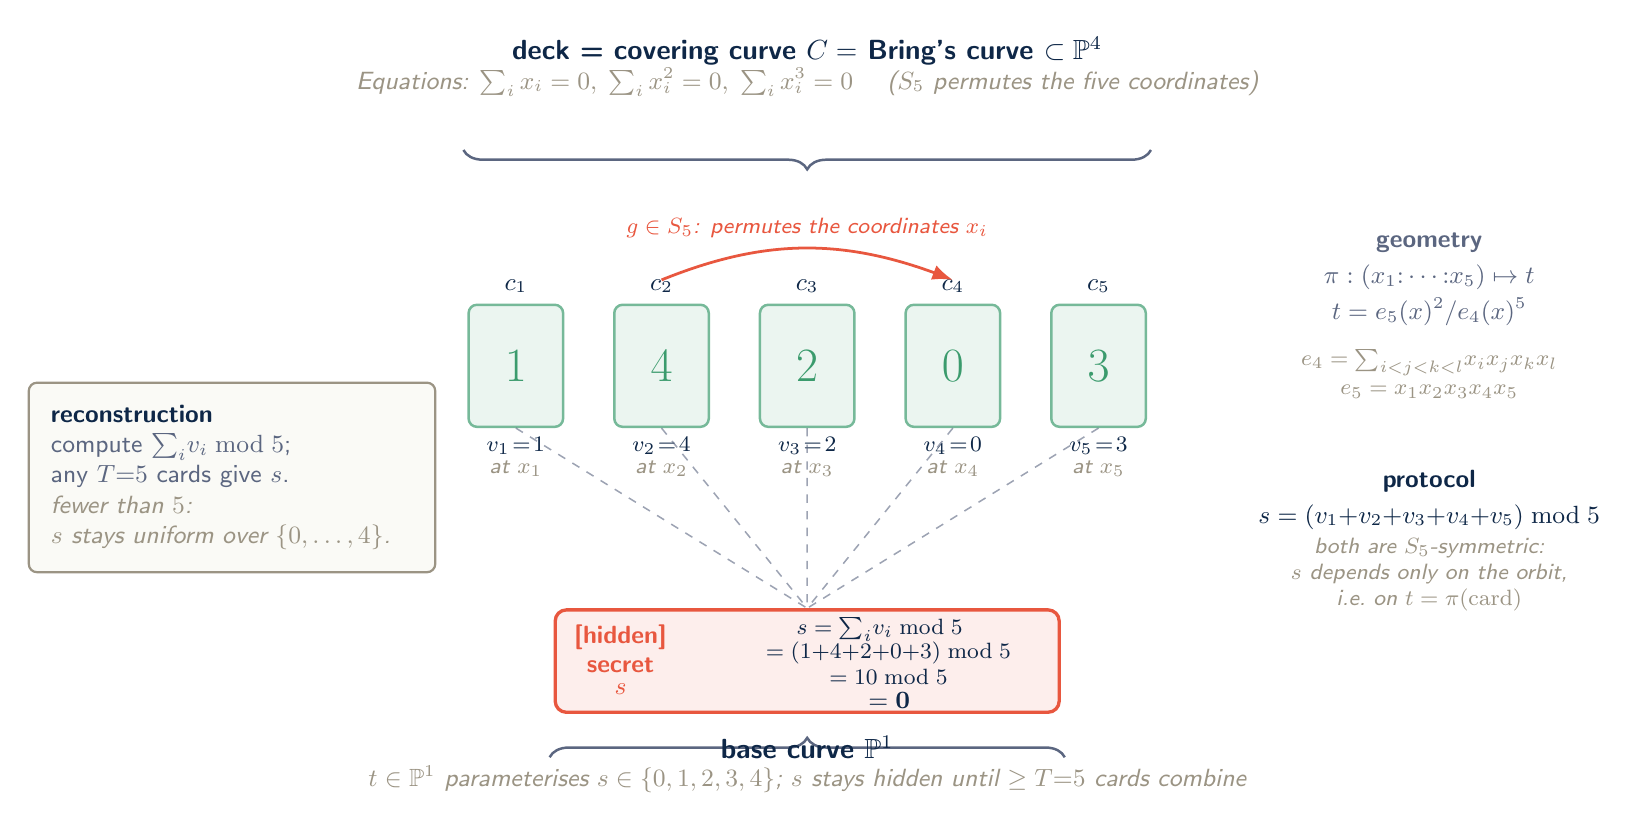
\begin{tikzpicture}[
  % Cards now have no suits; the big number inside is the share value v_i.
  card/.style={
    rectangle, rounded corners=3pt, draw=cgreen!70, fill=cgreen!10,
    line width=0.9pt, minimum width=1.20cm, minimum height=1.55cm, inner sep=0pt
  },
  secretbox/.style={
    rectangle, rounded corners=4pt, draw=corange, fill=corange!10,
    line width=1.2pt, minimum width=6.4cm, minimum height=1.30cm, inner sep=4pt
  },
  marrow/.style={dashed, draw=cslate, line width=0.55pt, opacity=0.6},
  gcurve/.style={-{Latex[length=2.6mm]}, draw=corange, line width=1.0pt},
  cbrace/.style={decorate, decoration={brace, amplitude=7pt}, line width=0.9pt, draw=cslate},
  font=\sffamily
]

% ============================================================
% Five neutral cards.  Each holds a concrete share value v_i in {0,...,4}.
% Example: (v_1,...,v_5) = (1,4,2,0,3), chosen so s = (Σ v_i) mod 5 = 0.
\node[card] (c1) at (0*1.85, 3.1) {};
\node[card] (c2) at (1*1.85, 3.1) {};
\node[card] (c3) at (2*1.85, 3.1) {};
\node[card] (c4) at (3*1.85, 3.1) {};
\node[card] (c5) at (4*1.85, 3.1) {};

% c_i index labels (small, above each card)
\foreach \i in {1,...,5} {
  \node[cnavy, font=\sffamily\bfseries\small] at ($(c\i.north)+(0,0.22)$) {$c_{\i}$};
}

% Big v_i values, centred inside each card
\node[cgreen, font=\sffamily\bfseries\LARGE] at (c1.center) {$1$};
\node[cgreen, font=\sffamily\bfseries\LARGE] at (c2.center) {$4$};
\node[cgreen, font=\sffamily\bfseries\LARGE] at (c3.center) {$2$};
\node[cgreen, font=\sffamily\bfseries\LARGE] at (c4.center) {$0$};
\node[cgreen, font=\sffamily\bfseries\LARGE] at (c5.center) {$3$};

% Below each card: explicit "v_i = ..." label and the coordinate x_i it sits over
\node[cnavy, font=\sffamily\bfseries\footnotesize] at ($(c1.south)+(0,-0.22)$) {$v_{1}\!=\!1$};
\node[cnavy, font=\sffamily\bfseries\footnotesize] at ($(c2.south)+(0,-0.22)$) {$v_{2}\!=\!4$};
\node[cnavy, font=\sffamily\bfseries\footnotesize] at ($(c3.south)+(0,-0.22)$) {$v_{3}\!=\!2$};
\node[cnavy, font=\sffamily\bfseries\footnotesize] at ($(c4.south)+(0,-0.22)$) {$v_{4}\!=\!0$};
\node[cnavy, font=\sffamily\bfseries\footnotesize] at ($(c5.south)+(0,-0.22)$) {$v_{5}\!=\!3$};

\node[cmuted, font=\sffamily\itshape\footnotesize] at ($(c1.south)+(0,-0.52)$) {at $x_{1}$};
\node[cmuted, font=\sffamily\itshape\footnotesize] at ($(c2.south)+(0,-0.52)$) {at $x_{2}$};
\node[cmuted, font=\sffamily\itshape\footnotesize] at ($(c3.south)+(0,-0.52)$) {at $x_{3}$};
\node[cmuted, font=\sffamily\itshape\footnotesize] at ($(c4.south)+(0,-0.52)$) {at $x_{4}$};
\node[cmuted, font=\sffamily\itshape\footnotesize] at ($(c5.south)+(0,-0.52)$) {at $x_{5}$};

% Curved monodromy arrow: a permutation in S_5
\draw[gcurve, bend left=22] ($(c2.north)+(0,0.30)$) to
  node[midway, above=0pt, font=\sffamily\itshape\footnotesize, color=corange]
       {$g \in S_{5}$: permutes the coordinates $x_{i}$}
  ($(c4.north)+(0,0.30)$);

% Brace + title block above the deck
\draw[cbrace] ($(c5.north east)+(0.05,1.95)$) -- ($(c1.north west)+(-0.05,1.95)$);
\node[cnavy,  font=\sffamily\bfseries] at (3.7, 7.10)
  {deck = covering curve $C =$ Bring's curve $\subset \mathbb{P}^{4}$};
\node[cmuted, font=\sffamily\itshape\small] at (3.7, 6.70)
  {Equations: $\sum_{i} x_{i}=0,\;\sum_{i} x_{i}^{2}=0,\;\sum_{i} x_{i}^{3}=0$
   \quad ($S_{5}$ permutes the five coordinates)};

% ============================================================
% Side annotations: the two formulas that connect curve <-> secret.
% Geometric quotient (curve side) and protocol recovery (secret side) shown
% explicitly so the encoding mechanism is visible.

\node[cslate, font=\sffamily\itshape\small, align=center] at (11.6, 4.2)
  {\textbf{geometry}\\[2pt]
   $\pi : (x_{1}{:}\cdots{:}x_{5}) \mapsto t$\\[2pt]
   $t = e_{5}(x)^{2} / e_{4}(x)^{5}$};
\node[cmuted, font=\sffamily\itshape\footnotesize, align=center] at (11.6, 3.0)
  {$e_{4} = {\sum}_{i<j<k<l} x_{i}x_{j}x_{k}x_{l}$\\[1pt]
   $e_{5} = x_{1}x_{2}x_{3}x_{4}x_{5}$};

\node[cnavy, font=\sffamily\itshape\small, align=center] at (11.6, 1.4)
  {\textbf{protocol}\\[2pt]
   $s = (v_{1}{+}v_{2}{+}v_{3}{+}v_{4}{+}v_{5}) \bmod 5$};
\node[cmuted, font=\sffamily\itshape\footnotesize, align=center] at (11.6, 0.45)
  {both are $S_{5}$-symmetric:\\
   $s$ depends only on the orbit,\\
   i.e.\ on $t = \pi(\mathrm{card})$};

% ============================================================
% Lower row: secret on the base curve.  Concrete value: s = 0.
\node[secretbox] (s) at (3.7, -0.65) {};
\node[corange, font=\sffamily\bfseries\small] at ($(s.west)+(0.85,0.30)$) {[hidden]};
\node[corange, font=\sffamily\bfseries\small] at ($(s.west)+(0.85,-0.05)$) {secret};
\node[corange, font=\sffamily\bfseries\small] at ($(s.west)+(0.85,-0.35)$) {$s$};
\node[cnavy,   font=\sffamily\bfseries\footnotesize]
  at ($(s.east)+(-2.30,0.40)$) {$s = {\sum}_{i} v_{i} \bmod 5$};
\node[cnavy,   font=\sffamily\bfseries\footnotesize]
  at ($(s.east)+(-2.30,0.10)$) {$\phantom{s}= (1{+}4{+}2{+}0{+}3) \bmod 5$};
\node[cnavy,   font=\sffamily\bfseries\footnotesize]
  at ($(s.east)+(-2.30,-0.20)$) {$\phantom{s}= 10 \bmod 5$};
\node[cnavy,   font=\sffamily\bfseries\small]
  at ($(s.east)+(-2.30,-0.50)$) {$\phantom{s}= \mathbf{0}$};

% Brace + label below the base
\draw[cbrace] ($(s.south west)+(-0.05,-0.55)$) -- ($(s.south east)+(0.05,-0.55)$);
\node[cnavy, font=\sffamily\bfseries] at (3.7, -1.75) {base curve $\mathbb{P}^{1}$};
\node[cmuted, font=\sffamily\itshape\small] at (3.7, -2.15)
  {$t \in \mathbb{P}^{1}$ parameterises $s \in \{0,1,2,3,4\}$;
   $s$ stays hidden until $\ge T{=}5$ cards combine};

% Dashed lines: each card contributes its v_i to the sum that defines s.
% Labels along three of the lines show the sum being assembled.
\foreach \i in {1,...,5} {
  \draw[marrow] (c\i.south) -- (s.north);
}

% Reconstruction callout on the left
\node[draw=cmuted, fill=ccream, rounded corners=3pt, line width=0.8pt,
      inner sep=8pt, align=left, anchor=north west, font=\sffamily\small,
      text width=4.6cm]
  at (-6.2, 2.9)
  {\textcolor{cnavy}{\textbf{reconstruction}} \\
   \textcolor{cslate}{compute ${\sum}_{i} v_{i}\bmod 5$;} \\
   \textcolor{cslate}{any $T{=}5$ cards give $s$.} \\
   \textcolor{cmuted}{\textit{fewer than $5$:}} \\
   \textcolor{cmuted}{\textit{$s$ stays uniform over $\{0,\dots,4\}$.}}};

\end{tikzpicture}
\end{document}
